\documentclass[tikz]{standalone}

\usepackage{amsmath}
\usepackage{circuitikz}
\usepackage{siunitx}

\let\Re\undefined
\DeclareMathOperator{\Re}{\operatorname{Re}}

\begin{document}
	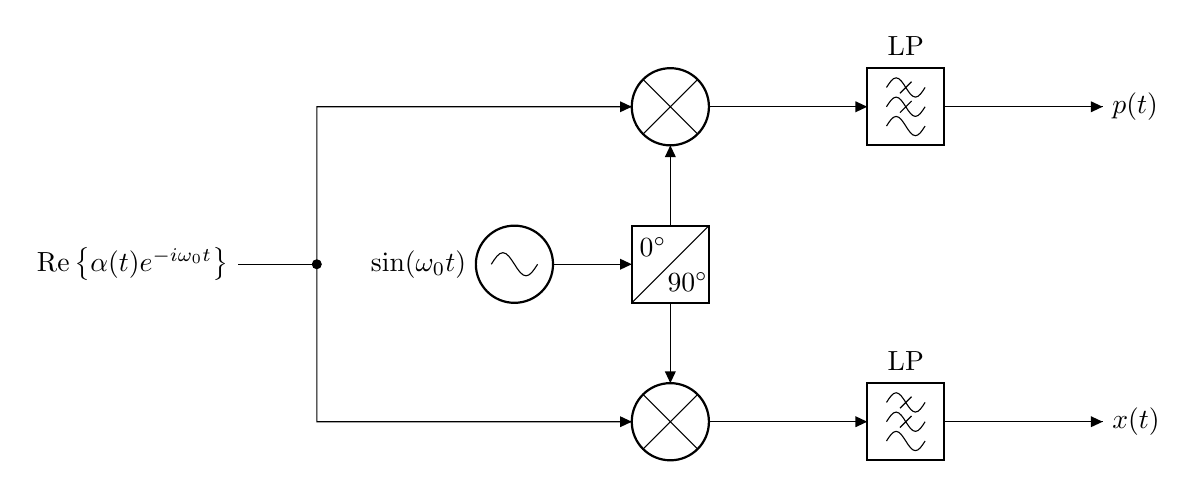
\begin{tikzpicture}
		\draw (0,0) node[left]{$\Re\left\{\alpha(t)e^{-i\omega_0t}\right\}$} to[short] ++(1,0)
            node[circ](term){};
        \draw (term) to[short] ++(0,2) to[short] ++(4,0) node[inputarrow]{} node[mixer, anchor=west](mixeru){};
        \draw (term) to[short] ++(0,-2) to[short] ++(4,0) node[inputarrow]{} node[mixer, anchor=west](mixerd){};
        \draw (term) ++(3,0) node[oscillator, label={left:$\sin(\omega_0t)$}](osc){};
        \draw (osc.west) (osc-|mixeru) node[twoportsplitshape, circuitikz/t1=$\SI{0}{\degree}$, circuitikz/t2=$\SI{90}{\degree}$](split){};
        \draw (osc.east) to[short] (split.west) node[inputarrow]{};
        \draw (split.north) to[short] (mixeru.south) node[inputarrow, rotate=90]{};
        \draw (split.south) to[short] (mixerd.north) node[inputarrow, rotate=-90]{};
        \draw (mixeru.east) to[short] ++(1,0) to[lowpass, >, l=LP] ++(3,0) to[short] ++(1,0) node[inputarrow]{} node[right]{$p(t)$};
        \draw (mixerd.east) to[short] ++(1,0) to[lowpass, >, l=LP] ++(3,0) to[short] ++(1,0) node[inputarrow]{} node[right]{$x(t)$};
	\end{tikzpicture}
\end{document}
